\documentclass[10pt]{article} %indicating type of document, font size
\usepackage[letterpaper, margin=1in]{geometry} %package that allows changes in margins and header/footers
\usepackage{hyperref}
\usepackage[pdftex]{graphicx}  
%\usepackage[leftcaption]{sidecap} %package for adding side captions
\usepackage{sidecap}
\usepackage[labelsep=period]{caption} %package for formatting figure captions, separation between figure number and caption is period
\sidecaptionvpos{figure}{c} %position side caption
\usepackage{lipsum}
\usepackage{indentfirst}
\usepackage{color}
\usepackage{multirow}
\usepackage[document]{ragged2e}
\begin{document}





%Triglochin maritima
%-------------------------------------------------------------------
\begin{SCfigure}
 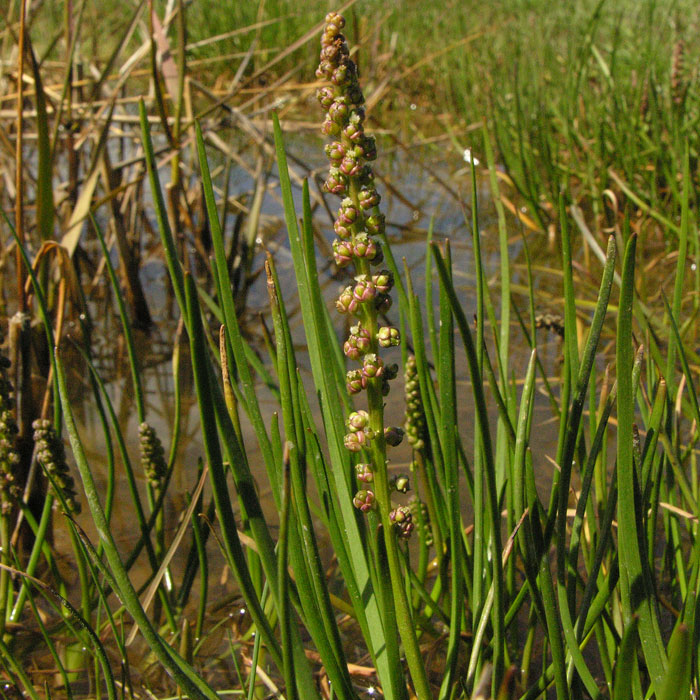
\includegraphics[width=80mm]{Triglochin01.jpg}
 \caption{{{\bf{Triglochin maritima, Sea arrowgrass}}\\- In Berkeley Marina, Crissy Field Northern waterfront, Pier 94\\
-Low zone of salt marsh, if high tide will be submerged\\
-narrow rounded leaf blades; 2-3 ft tall\\
-Flower/seed stalks tall, round seeds along stalk; may still have seeds}}
 \end{SCfigure}
%-------------------------------------------------------------------

%Triglochin maritima
%-------------------------------------------------------------------
\begin{SCfigure}
 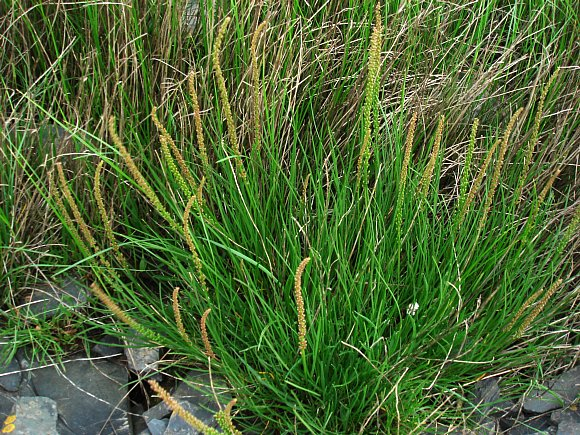
\includegraphics[width=80mm]{Triglochin04.jpg}
 \caption{{{\bf{Triglochin maritima, Sea arrowgrass}}\\- In Berkeley Marina, Crissy Field Northern waterfront, Pier 94\\
- Low zone of salt marsh, if high tide will be submerged\\
- narrow rounded leaf blades; 2-3 ft tall\\
- Flower/seed stalks tall, round seeds along stalk; may still have seeds\\**aka \emph{Lilaea Scilloides}; flowering quilwort}}
 \end{SCfigure}
%-------------------------------------------------------------------

%Triglochin maritima
%-------------------------------------------------------------------
\begin{SCfigure}
 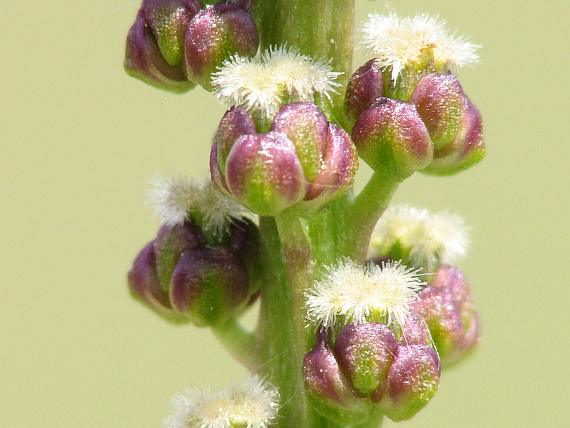
\includegraphics[width=80mm]{Triglochin03.jpg}
 \caption{{{\bf{Triglochin maritima, Sea arrowgrass}}\\- In Berkeley Marina, Crissy Field Northern waterfront, Pier 94\\
- Low zone of salt marsh, if high tide will be submerged\\
- narrow rounded leaf blades; 2-3 ft tall\\
- Flower/seed stalks tall, round seeds along stalk; may still have seeds\\**aka \emph{Lilaea Scilloides}; flowering quilwort}}
 \end{SCfigure}
%-------------------------------------------------------------------

%Ruppia maritima
%-------------------------------------------------------------------
\begin{SCfigure}
 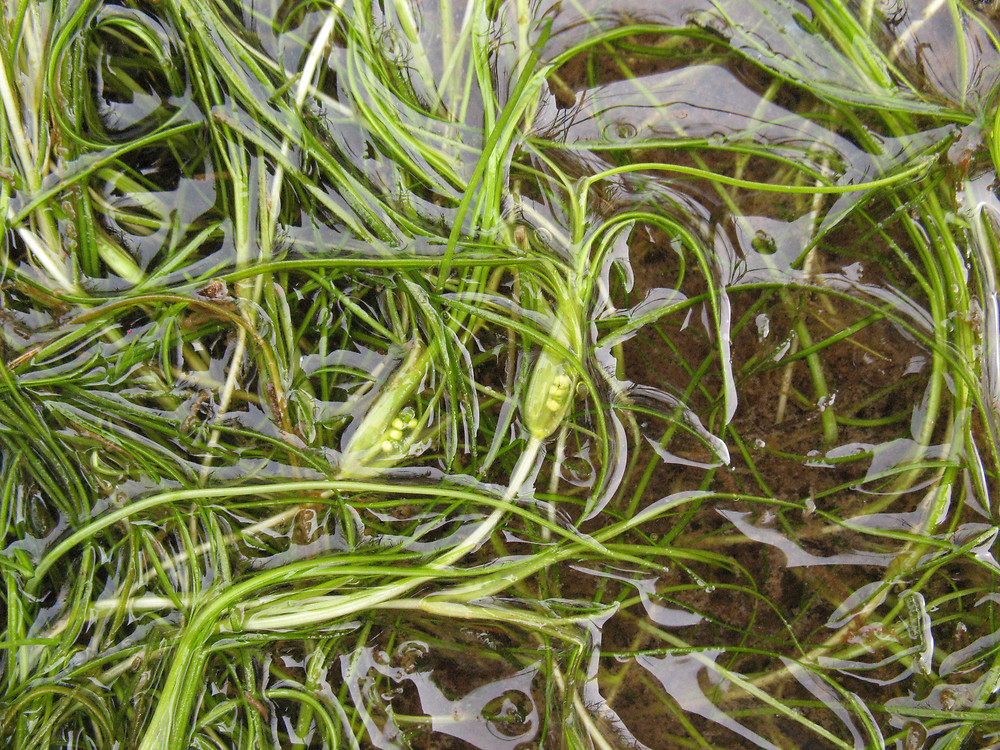
\includegraphics[width=80mm]{Ruppia04.jpg}
 \caption{{{\bf{Ruppia maritima; widgeongrass, ditch-grass and tassel pondweed}}\\- Mare Island\\- Thin threadlike leaves, shallow roots, coiled inflorescence each with 2 flowers; fruits are drupelets\\- Long, narrow, alternate leaves are less than 1 mm wide. Stipular sheaths, less than 7 cm long, are completely fused to the leaf and often broadly clasp the stem\\- Tiny flowers (3-5 mm across), lack petals and sepals, and occur in pairs on stalks. Pollination often occurs underwater or at the waters surface. Once pollinated, the flower stalk coils.\\- Fruits are dark colored, egg to pear-shaped, symmetrical to highly asymmetrical achene is 1.5 to 2 mm long and occurs in a cluster. Each fruit is on individual stalks, but all are connected to a long flowering stalk (peduncle) }}
 \end{SCfigure}
%-------------------------------------------------------------------

%Ruppia maritima 02
%-------------------------------------------------------------------
\begin{SCfigure}
 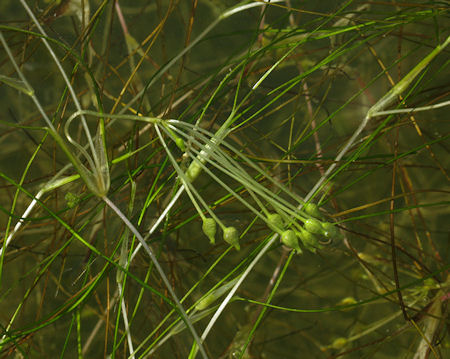
\includegraphics[width=80mm]{Ruppia02.jpg}
 \caption{{{\bf{Ruppia maritima; widgeongrass, ditch-grass and tassel pondweed}}\\-Mare Island\\- Thin threadlike leaves, shallow roots, coiled inflorescence each with 2 flowers; fruits are drupelets\\ - Long, narrow, alternate leaves are less than 1 mm wide. Stipular sheaths, less than 7 cm long, are completely fused to the leaf and often broadly clasp the stem\\- Tiny flowers (3-5 mm across), lack petals and sepals, and occur in pairs on stalks. Pollination often occurs underwater or at the waters surface. Once pollinated, the flower stalk coils.\\- Fruits are dark colored, egg to pear-shaped, symmetrical to highly asymmetrical achene is 1.5 to 2 mm long and occurs in a cluster. Each fruit is on individual stalks, but all are connected to a long flowering stalk (peduncle) }}
 \end{SCfigure}
%-------------------------------------------------------------------

%Alisma trivale%-------------------------------------------------------------------
\begin{SCfigure}
 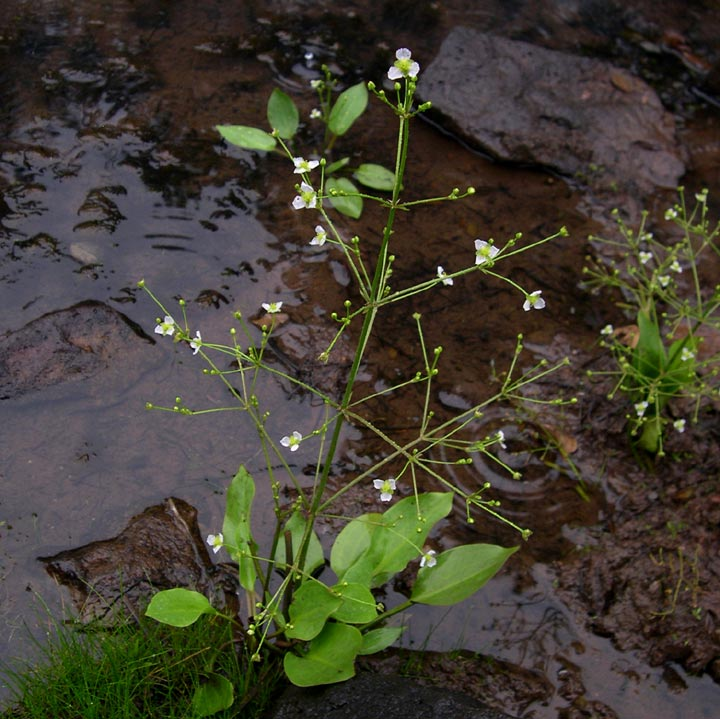
\includegraphics[width=80mm]{Alisma01.jpg}
 \caption{{{\bf{Alisma triviale, Water Plantain}}\\- Freshwater, marshes muddy shorelines, ditches, shallow lakes or slow moving streams\\- Marin County, Mt. Tamalpais, Bullfrog Road; sampled 2013\\- Likely in bloom }}
 \end{SCfigure}
%-------------------------------------------------------------------


%Alisma trivale%-------------------------------------------------------------------
\begin{SCfigure}
 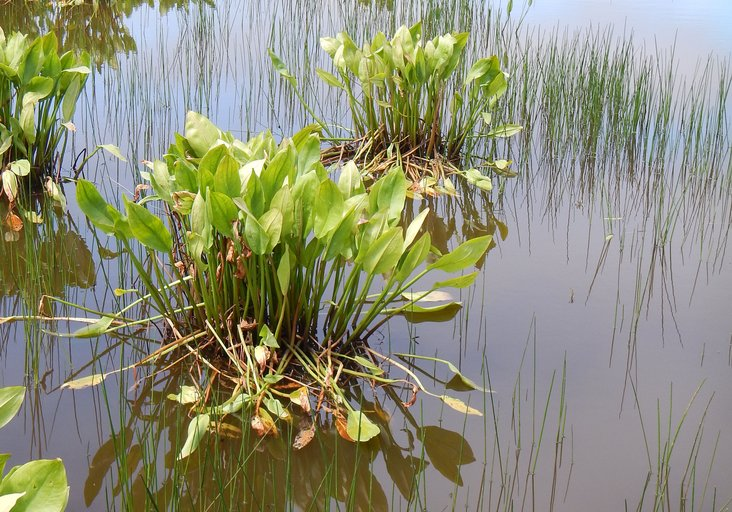
\includegraphics[width=80mm]{Alisma02.jpg}
 \caption{{{\bf{Alisma triviale; Water Plantain}}\\-Leaves growing from base of plant; made up of one segment; blade 30-350 mm\\- Flowers are white with three petals/sepals\\- Does not have underwater leaves (generally) }}
 \end{SCfigure}
%-------------------------------------------------------------------

%Alisma trivale%-------------------------------------------------------------------
\begin{SCfigure}
 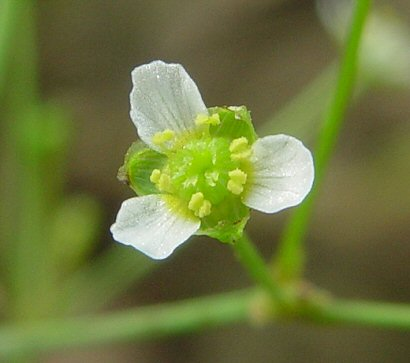
\includegraphics[width=80mm]{Alisma03.jpg}
 \caption{{{\bf{Alisma triviale; Water Plantain}}\\-Leaves growing from base of plant; made up of one segment; blade 30-350 mm\\- Flowers are white with three petals/sepals\\- Does not have underwater leaves (generally) }}
 \end{SCfigure}
%-------------------------------------------------------------------

%Echinodorus berteroi%-------------------------------------------------------------------
\begin{SCfigure}
 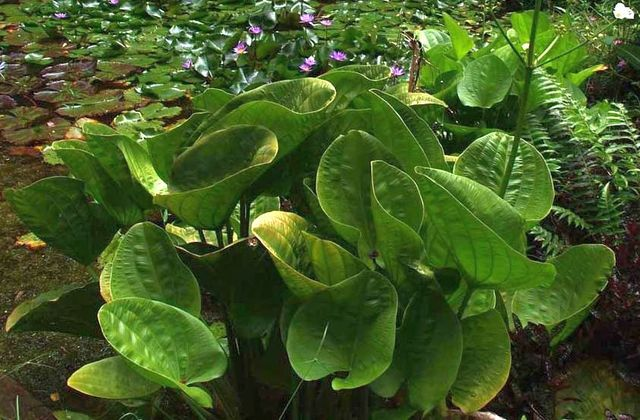
\includegraphics[width=80mm]{Echinodorus01.jpg}
 \caption{{{\bf{Echinodorus berteroi; Upright burhead, Cellophane sword}}\\- Freshwater, can also be terrestrial; Stafford Lake, Marin County; American River in Sacramento\\- Leaves can be submerged or not, directly off of plant; 10-45 cm long x 0.5-4 cm wide; leaves can appear mosaic like in color; ovate leaves\\- Upright stem with compound inflorescence, white flowers, 12 stamens\\- nutlets are grey-brown with 2 winged ribs alternating with 3 non-winged ribs}}
 \end{SCfigure}
%-------------------------------------------------------------------


%Echinodorus berteroi%-------------------------------------------------------------------
\begin{SCfigure}
 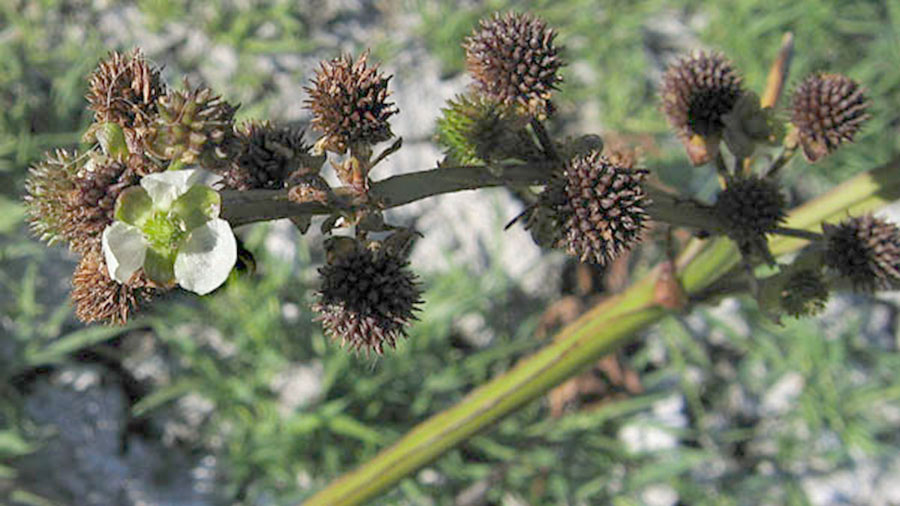
\includegraphics[width=80mm]{Echinodorus02.jpg}
 \caption{{{\bf{Echinodorus berteroi; Upright burhead, Cellophane sword}}\\- Freshwater, can also be terrestrial; Stafford Lake, Marin County; American River in Sacramento\\- Leaves can be submerged or not, directly off of plant; 10-45 cm long x 0.5-4 cm wide; leaves can appear mosaic like in color; ovate leaves\\- Upright stem with compound inflorescence, white flowers, 12 stamens\\- nutlets are grey-brown with 2 winged ribs alternating with 3 non-winged ribs}}
 \end{SCfigure}
%-------------------------------------------------------------------

%Echinodorus berteroi%-------------------------------------------------------------------
\begin{SCfigure}
 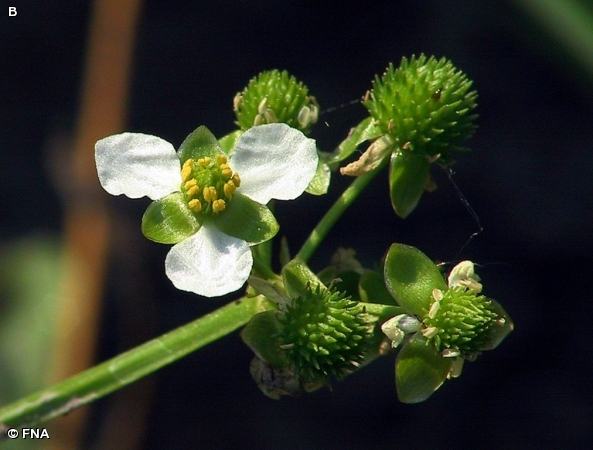
\includegraphics[width=80mm]{Echinodorus03.jpg}
 \caption{{{\bf{Echinodorus berteroi; Upright burhead, Cellophane sword}}\\- Freshwater, can also be terrestrial; Stafford Lake, Marin County; American River in Sacramento\\- Leaves can be submerged or not, directly off of plant; 10-45 cm long x 0.5-4 cm wide; leaves can appear mosaic like in color; ovate leaves\\- Upright stem with compound inflorescence, white flowers, 12 stamens\\- nutlets are grey-brown with 2 winged ribs alternating with 3 non-winged ribs}}
 \end{SCfigure}
%-------------------------------------------------------------------

%Potamogeton filiformis%-------------------------------------------------------------------
\begin{SCfigure}
 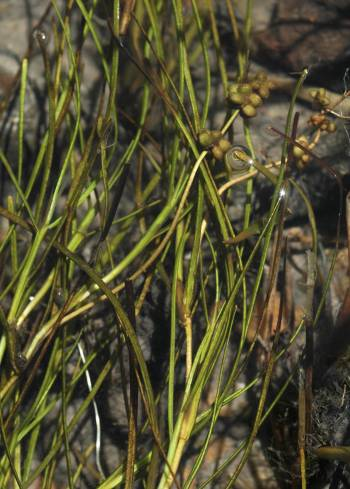
\includegraphics[width=80mm]{Potamogeton01.jpg}
 \caption{{{\bf{Potamogeton filiformis; aka Stuckenia filiformis; Threadleaved False Pondweed}}\\- Freshwater, confluence of Sacramento and San Joaquin Rivers; Brown Island north of Pittsburgh\\- Slender leaves, growth from rhizome}}
 \end{SCfigure}
%-------------------------------------------------------------------

%Potamogeton filiformis%-------------------------------------------------------------------
\begin{SCfigure}
 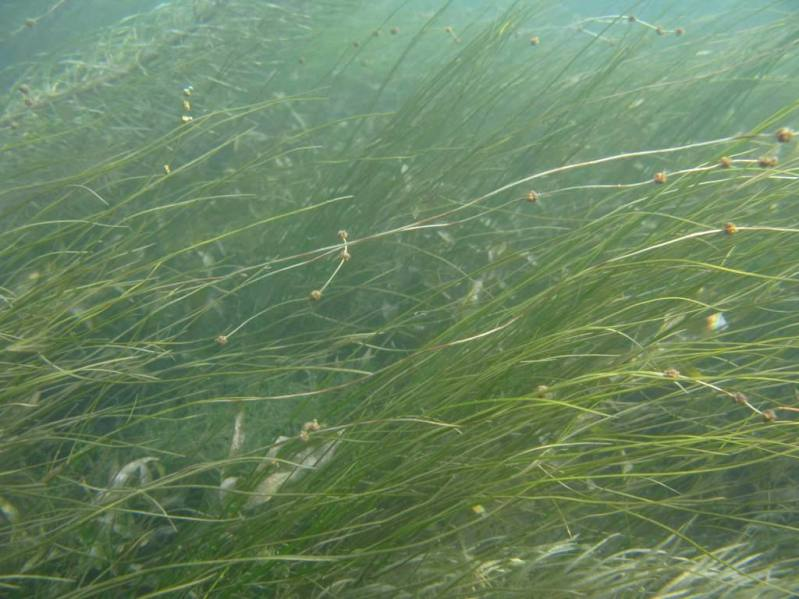
\includegraphics[width=80mm]{Potamogeton03.jpg}
 \caption{{{\bf{Potamogeton filiformis; aka Stuckenia filiformis; Threadleaved False Pondweed}}\\- Freshwater, confluence of Sacramento and San Joaquin Rivers; Brown Island north of Pittsburgh\\- Slender leaves, growth from rhizome}}
 \end{SCfigure}
%-------------------------------------------------------------------

%Potamogeton filiformis%-------------------------------------------------------------------
\begin{SCfigure}
 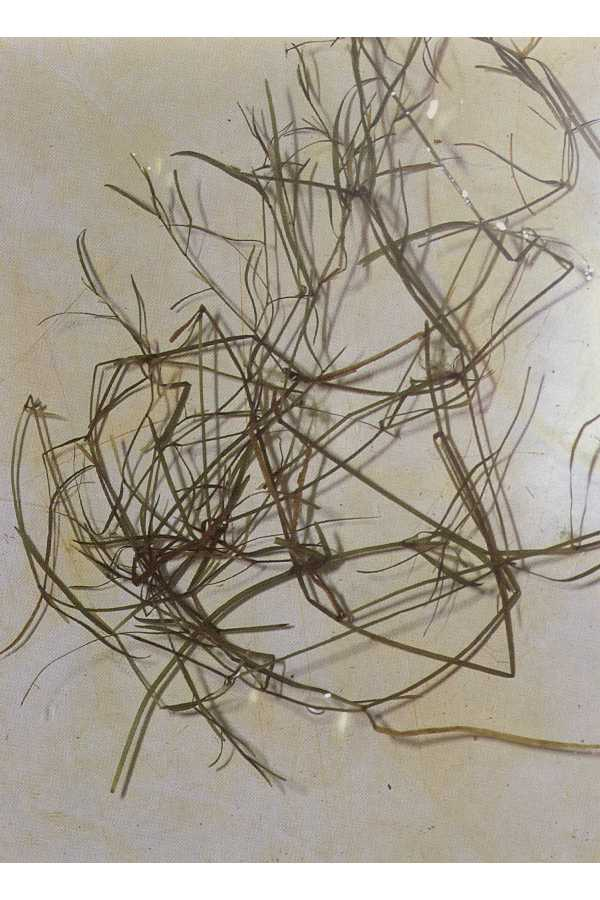
\includegraphics[width=80mm]{Potamogeton05.jpg}
 \caption{{{\bf{Potamogeton filiformis; aka Stuckenia filiformis; Threadleaved False Pondweed}}\\- Freshwater, confluence of Sacramento and San Joaquin Rivers; Brown Island north of Pittsburgh\\- Slender leaves, growth from rhizome}}
 \end{SCfigure}
%-------------------------------------------------------------------

%Sagittaria latifolia%-------------------------------------------------------------------
\begin{SCfigure}
 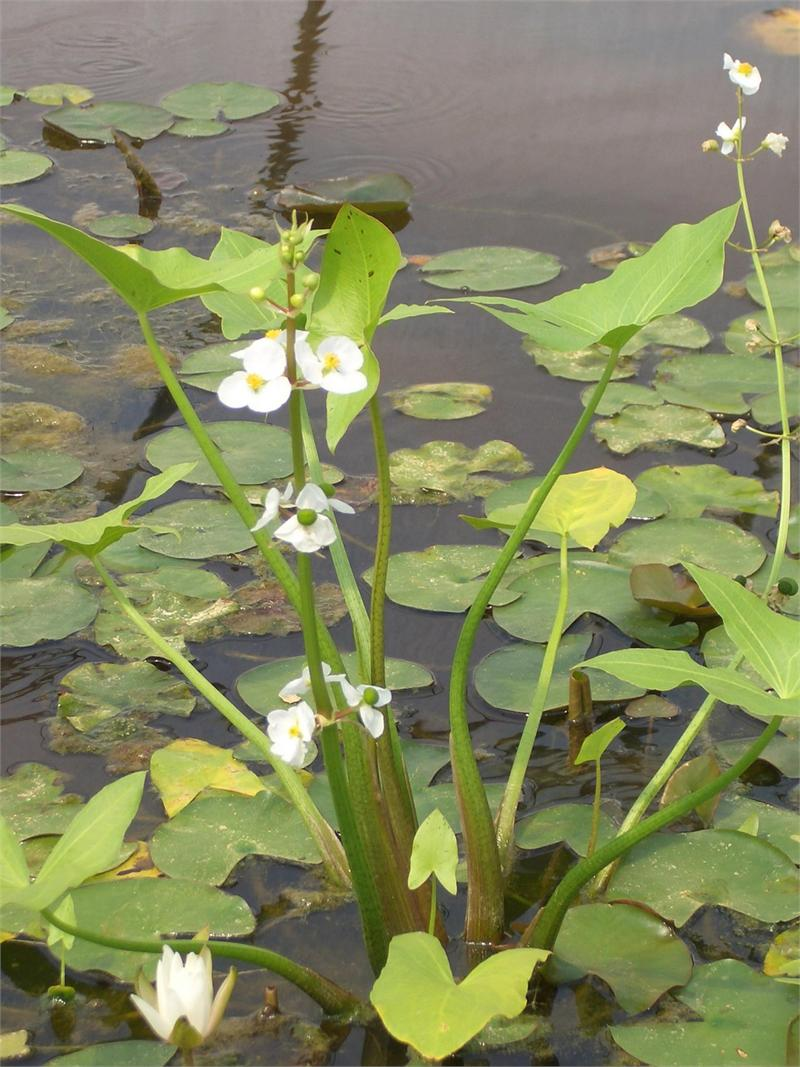
\includegraphics[width=80mm]{Sagittaria01.jpg}
 \caption{{{\bf{Sagittaria latifolia; Broadleaf Arrowhead, Duck Potato}}\\- Freshwater, usually growing in dense clumps in mud, shallow water, or fully saturated soil\\- Perennial; up to 3 ft tall\\- leaves with long petioles, arrowhead shaped, pointed up\\- White flowers, three petals, 3 sepals, 6+stamens, male and female parts on diff. flowers}}
 \end{SCfigure}
%-------------------------------------------------------------------

%-------------------------------------------------------------------
\begin{SCfigure}
 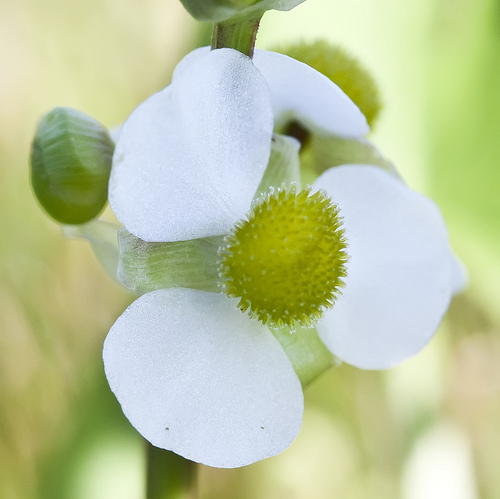
\includegraphics[width=80mm]{Sagittaria03.jpg}
 \caption{{{\bf{Sagittaria latifolia; Broadleaf Arrowhead, Duck Potato}}\\- Freshwater, usually growing in dense clumps in mud, shallow water, or fully saturated soil\\- Perennial; up to 3 ft tall\\- leaves with long petioles, arrowhead shaped, pointed up\\- White flowers, three petals, 3 sepals, 6+stamens, male and female parts on diff. flowers}}
 \end{SCfigure}
%-------------------------------------------------------------------

\end{document}